% ----------------------------------------------------------------------------
% Copyright (c) 2016 - 2020 by Burkhardt Renz. All rights reserved.
% Die Vorlage für eine Abschlussarbeit in der Informatik am Fachbereich
% MNI der THM ist lizenziert unter einer Creative Commons
% Namensnennung-Nicht kommerziell 4.0 International Lizenz.
%
% Id:$
% ----------------------------------------------------------------------------

\chapter{Elemente im Text}

Der Text dieses Kapitels steht in \verb=elemente.tex= und bezieht auch
auf diese Datei.

\section{Typografische Elemente}

Im laufenden Text kann man alles Mögliche machen. Gute Typografie geht
mit diesen Möglichkeiten sparsam um. Was in Texten der Informatik oft
vorkommt ist die \emph{Hervorhebung} mit dem Befehl \verb=\emph=. Man
verwendet kursive Schrift auch für fremdsprachige Worte im Text, etwa
\textit{digital typography}.
Für Schlüsselworte, Befehle der Kommandozeile u.ä. nimmt man gerne einen
passenden Zeichensatz, etwa \texttt{make vorlage.pdf}. 

Das Paket \verb=csquotes= sorgt dafür dass Anführungszeichen
typografisch korrekt verwendet werden. Im Deutschen werden die
\enquote{Gänsefüßchen} nämlich anders als die angelsächsischen
\foreignquote{english}{quotation marks} gesetzt.

Mehr über das Setzen von Text findet man in \cite{lkurz15}.

\section{Referenzen und Links}

Verweise auf die Literatur macht man mit dem Befehl \verb=\cite=.
Braucht man Querverweise auf Abschnitte im Text oder Abbildungen etc.,
so versieht man das Verweisziel mit einem \verb=\label= und verweist
dann mit \verb=\ref= oder \verb=\pageref=. Mehr dazu in
\cite[S.50]{partosch15}.

Links auf Quellen im Internet werden durch den Befehl \verb=\url=
angegeben und dadurch in PDF \enquote{anklickbar}, etwa wie
\url{https://tug.org/mactex/src/WelcomeToMacTeX.pdf}.

\section{Abbildungen}

\begin{figure}[!htb]
	\centering
	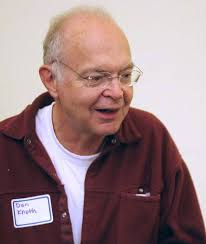
\includegraphics[width=.4\textwidth]{img/knuth.jpg}
	\caption{Donald Knuth}
	\label{fig:knuth}
\end{figure}


\begin{figure}[!htb]
	\centering
	\includegraphics[width=.4\textwidth]{img/783px-Test-Logo.svg}
	\caption{Test}
	\label{fig:test}
\end{figure}

Abbildungen bindet man mit \verb=\includegraphics= in einer Umgebung
\verb=figure= ein.
Man kann dann im Text auf die Abbildung \ref{fig:knuth} verweisen.
Man muss beachten, dass die Abbildung in einer sogenannten
\enquote{fließenden} Umgebung eingebunden wird, d.h. beim Setzen des
Dokuments bestimmt \TeX, an welcher Stelle genau im Dokument die
Abbildung erscheint.

Wie man an diesem Beispiel sieht, kann man beliebige Abbildungen etwa
\verb=jpg= wie in diesem Beispiel, aber auch \verb=pdf= einbinden. Man
kann also Abbildungen mit einem Grafikprogramm erstellen, als
\verb=pdf= speichern und dann einbinden.

\newcommand{\tikz}{Ti\emph{k}Z}

Es gibt aber auch \tikz\ (= \tikz\ ist kein Zeichenprogramm), das der
deutsche Informatiker Till Tantau entwickelt hat. Damit ist es möglich,
Abbildungen zu \enquote{programmieren}. Die Projektseite von \tikz\ ist
\url{https://sourceforge.net/projects/pgf/}. Interessant sind auch
die Beispiele auf \url{http://www.texample.net/tikz/examples/}.

\section{Tabellen}

Tabellen werden in einer \enquote{fließenden} Umgebung namens
\verb=table= eingegeben. Der eigentliche Inhalt der Tabelle kommt in die
Umgebung \verb=tabular=.

\begin{table}[!htb]
	\centering
	\caption{Die Geschichte von \TeX\ und \LaTeX}
	\begin{tabular}{ r p{13cm}}
		\toprule
		Jahr & Entwicklung\\
		\midrule
		1977 & Donald Knuth beginnt mit der Entwicklung von \TeX.\\
		1985 & \LaTeX\ (mächtige Makros, die die Verwendung von \TeX\
			vereinfachen, in dem sie Struktur und Layout trennen) wird von
			Leslie Lamport in der Version 2.09 freigegeben.\\
		1986 & Feier der Fertigstellung von \TeX\ im Computer Museum in
		Boston\\
		1986 & Leslie Lamport veröffentlicht \emph{\LaTeX: A Document
			Preparation System}.\\
		1993 & \LaTeXe\\
		2000 & pdf\TeX\ (entwickelt von Hàn Thé Thành)\\
			?  & Nach dem Tod von Donald Knuth bekommt \TeX\ die Versionsnummer
			$\pi$.\\
		\bottomrule
	\end{tabular}
	\label{tbl:geschichte}
\end{table}

Wie man am Beispiel des \LaTeX-Texts der Tabelle  \ref{tbl:geschichte}
sieht, kann die Formatierung von Tabellen etwas \enquote{sperrig} sein.
Gut, dass man sich in einer der vielen Anleitungen dazu erkundigen kann,
z.B. in der \LaTeXe-Kurzbeschreibung \cite[S.23]{lkurz15}.

\section{Listings}

\verb=listings= ist ein Paket, das es erlaubt, Code-Beispiele in die
Abschlussarbeit zu setzen. Wie das Beispiel \ref{lst:datei} zeigt, kann
man auch externe Dateien einbinden und im Text verbatim einsetzen. In
diesem Fall kann der eingebundene Text auch in der Zeichenkodierung
\emph{utf8} sein, wohingegen dies bei direkt im Text geschriebenen
Codebeispielen nicht unterstützt wird.

\begin{lstlisting}[caption={Einbinden einer Quelldatei}\label{lst:datei}]
% Der Inhalt der Datei myclass.java wird verbatim hier eingefügt
\lstinputlisting[caption={Eine Java-Klasse}\label{lst:java}]{myclass.java}
\end{lstlisting}

Für Listings gibt es viele Optionen des Layouts, insbesondere ist es
möglich die Programmiersprache des eingebundenen Code-Beispiels
anzugeben, was dazu führt, dass Schlüsselworte, Bezeichner und Kommentare
der Sprache im Layout hervorgehoben werden.

\section{Mathematische Formeln}

Mathematisches kann man in den laufenden Text einbauen, wie etwa bei
folgender Definition:

Mit $k!$, der Fakultät einer natürlichen Zahl $k$ bezeichnet man das
Produkt $1 \cdot 2 \cdot \dotso \cdot k$.

Oft braucht man aber auch ganze Abschnitte im Mathematik-Modus, wie in
folgendem Beispiel:

		Die sogenannte Collatz-Folge\footnote{ nach Lothar Collatz,
		deutscher Mathematiker 1910 - 1990} zu einer natürlichen Zahl $n$
		wird folgendermaßen gebildet:

	\begin{align}
	  n_1 &= n \nonumber \\
		n_{i+1} &= \left\{ \begin{array}{l l}
	                   n_i/2      & \textrm{falls $n_i$ gerade}\\
										 3 n_i + 1  & \textrm{falls $n_i$ ungerade}
										 \end{array} \right. \nonumber
	\end{align}

	\medskip
										 
	Startet man etwa mit der Zahl $7$ erhält man

	\[7\ 22\ 11\ 34\ 17\ 52\ 26\ 13\ 40\ 20\ 10\ 5\ 16\ 8\ 4\ 2\ 1\ 4\ 2\ 1\ \dots\]

	Wie man sieht, geht die Folge schließlich in den Zyklus $1, 4, 2$
	über.  Die \emph{Collatz-Vermutung} besagt, dass dies für jeden
	Startwert $n$ der Fall ist, d.h.  jede Collatz-Folge erreicht
	irgendwann den Wert $1$.

Mehr über das Setzen von mathematischen Formeln steht in \cite[Kapitel 4]{lkurz15}.



% ----------------------------------------------------------------------------
